\chapter{Data Curation}\label{chap:data}

\section{Data organization into MOOCdb}

As previously mentioned, we focused on the Fall 2012 offering of 6.002x: Circuits and Electronics. edX provided the following raw data from the 6.002x course:

\begin{itemize}
\item A dump of click-stream data from student-browser and edX-server tracking logs in JSON format. For instance, every page visited by every student was stored as a server-side JSON (JavaScript Object Notation) event.
\item Forum posts, edits, comments and replies stored in a MongoDB collection. Note that passive forum data, such as how many views a thread received was not stored here and had to be inferred from the click-stream data.
\item Wiki revisions stored in a MongoDB collection. Again, passive views of the Wiki must be inferred from the click-stream data.
\item A dump of the MySQL production database containing student state information. For example, the database contained his/her final answer to a problem, along with its correctness. Note that the history of his submissions must be inferred from the click-stream data.
\item An XML file of the course calendar which included information like the release of content and the assignment deadlines.
\end{itemize}

\begin{figure}[ht!]
  \caption{Multiple data sources received from edX with their corresponding formats}\label{fig:data_layout}
  \centering
    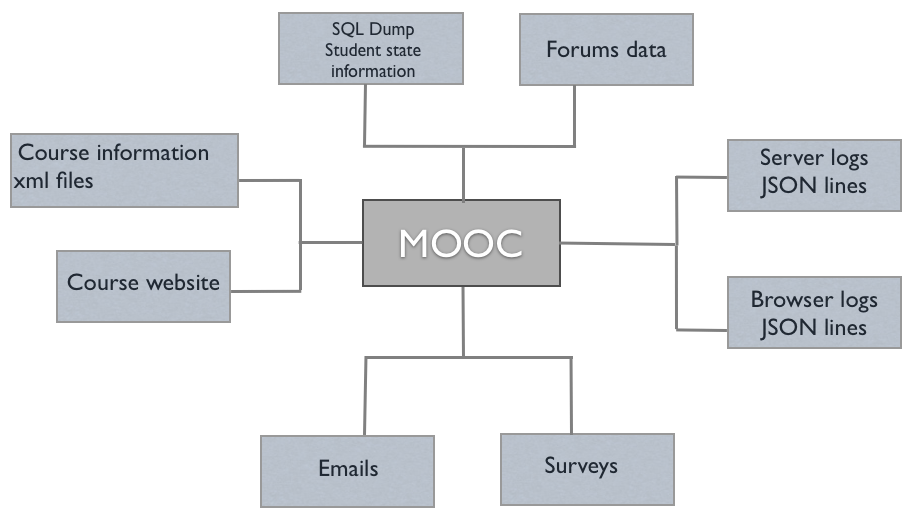
\includegraphics[width=1.0\textwidth]{figures/data_layout.png}
\end{figure}

Figure \ref{fig:data_layout} summarizes the raw data received.

This data included:
\begin{itemize}
\item 154,763 registered students
\item 17.8 million submission events
\item 132.3 million navigational events \footnote{We received more navigational events, but only 132.3 million were well formed enough to be reliably considered for this thesis. }
\item $\sim$90,000 forum posts
\end{itemize}

To analyze this data at scale, as well as write reusable analysis scripts, we first organized the data into a schema designed to capture pertinent information. The resulting database schema, MOOCdb, is designed to capture MOOC data across platforms thereby promoting collaboration among MOOC researchers. MOOCdb utilizes a large series of  scripts to pipe the 6.002x raw data into a standardized schema. More about MOOCdb can be found in the MOOCdb Tech report, but the details are outside the scope of this thesis \cite{tr}.

Through the labor intensive process of piping the raw data into a schematized database, we were able to significantly reduce the data size in terms of disk space. The original $\sim$70GB of raw data was reduced to a $\sim$7GB MOOCdb through schema normalization. The transformation was crucial in order to load the entire database into RAM enabling prompt queries and feature extractions. Figure~\ref{fig:data_reduction} shows a snapshot of the original JSON transactional data transformed into a normalized schema.

\begin{figure}[ht!]
  \caption{Piping data into MOOCdb}\label{fig:data_reduction}
  \centering
    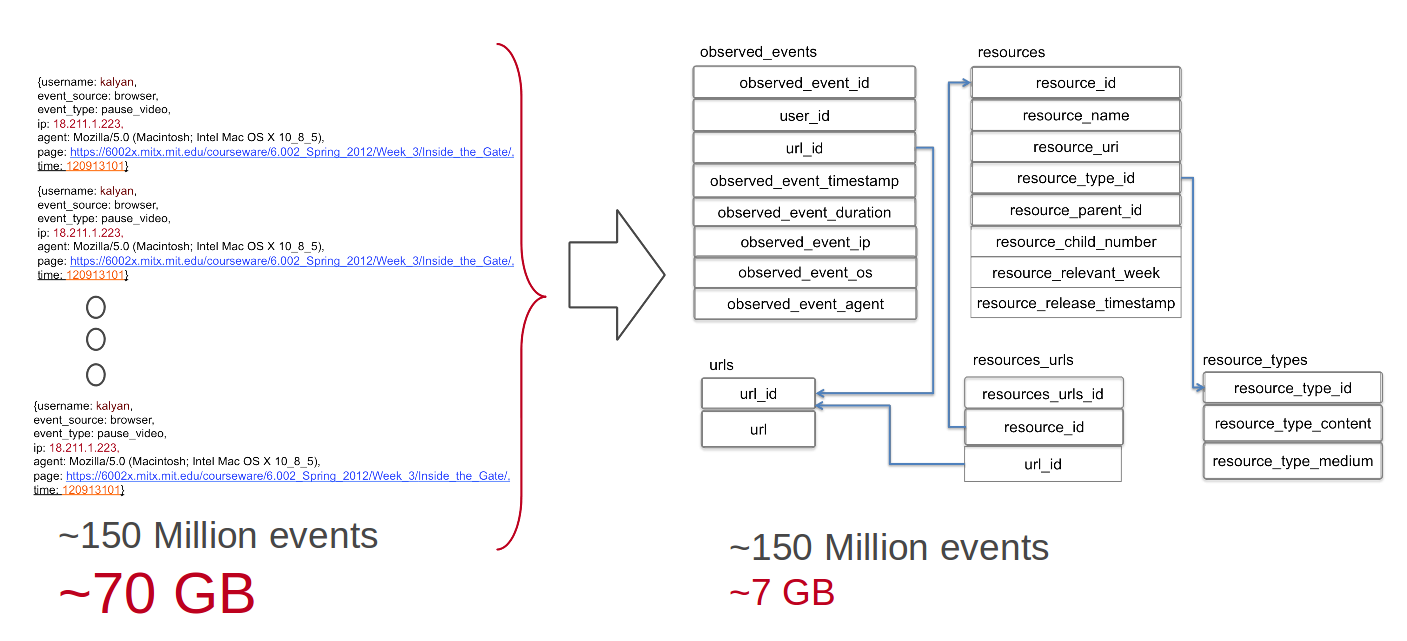
\includegraphics[width=1.0\textwidth]{figures/data_reduction.png}
\end{figure}

\section{Prediction problem assumptions}
We made several assumptions to more precisely define the \sti prediction problem and interpret the data. These assumptions include time-slice delineation and defining persistence (\sti) as the event we attempt to predict.

\subsection{Time-slice delineation}
Temporal prediction of a future event requires us to assemble explanatory variables along a time axis. This axis is subdivided to express the time-varying behavior of variables so they can be used for explanatory purposes. In 6.002x, course content was assigned and due on a weekly basis, where each week corresponded to a module. Owing to the regular modular structure, we decided to define time slices as weekly units. Time slices started the first week in which course content was offered, and ended in the fifteenth week, after the final exam had closed.

\subsection{Stopout definition}
The next question we had to address was our definition of stopout. We considered defining it by the student's last interaction in the course, regardless of the nature of the interaction. This is the approach taken by Balakrishnan in his \sti analysis \cite{balakrishnan2013predicting}. However, Balakrishnan's definition yields noisy results because it gives equal weight to a passive interaction (viewing a lecture, accessing an assignment, viewing a Wiki etc) as it does to a pro-active interaction (submitting a problem, midterm, assignment etc). A student could stop submitting assignments in the course after week 2, but continue to access the course pages and not be considered stopped out. Instead, we define the stop-out point as the time slice (week) a student fails to submit any further assignments or exercise problems. To illustrate, if a student submits his/her last assignment in the third module, he/she is considered to have stopped-out at week four. A submission (or attempt) is a submission of any problem type (Homework, lab, exam etc.), as defined in MOOCdb. This definition narrows the research to students who consistently participate in the course by submitting assignments. Using this definition for \sti we extracted the week number when each student in the cohort stopped out.

Figure~\ref{fig:dropout_week} shows the distribution of \sti week for all 105,622 students who ever accessed the course. Of these, 52,683 students stopped out on week one. These students never submitted an assignment, and are never considered in the rest of our analysis. Another large student drop off point is in week 15, the last week of the course. Many of these students actually finished the course, but did so by submitting their final exam in week 14. This nuance presented itself because students had a range of time to start the final exam, and this range actually overlapped between weeks 14 and 15. Due to the nature of the final exam time range, we never attempt to predict week 15, and consider week 14 as the final week.

\begin{figure}[ht!]
  \caption{Stopout week distribution}\label{fig:dropout_week}
  \centering
    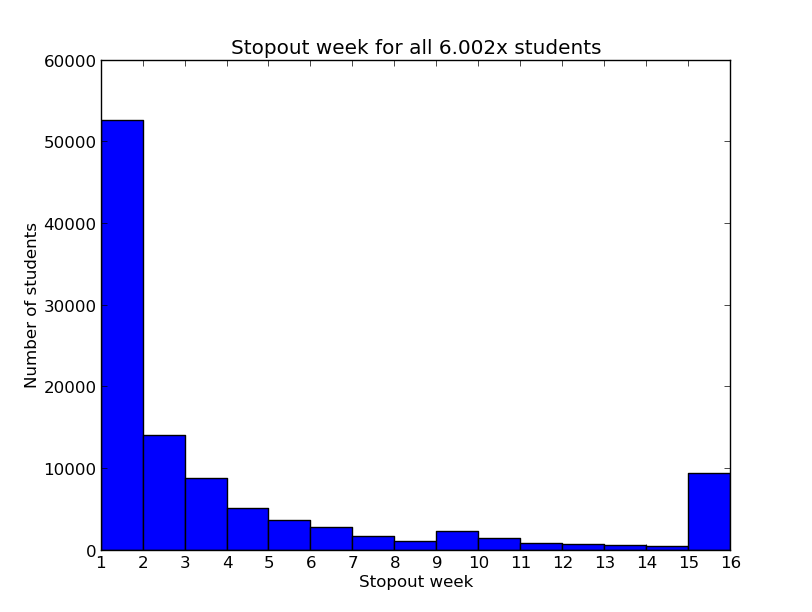
\includegraphics[width=1.0\textwidth]{figures/dropout_weeks.png}
\end{figure}

\subsection{Lead and Lag}
Lead represents how many weeks in advance to predict \sti. We assign the \sti label (\x{1}, 0 for \sti or 1 for persisted) of the lead week as the predictive problem label. Lag represents how many weeks of historical variables will be used to classify. For example, if we use a lead of 5 and a lag of 3, we would take the first 3 weeks of data to predict 5 weeks ahead. Thus, each training data point is a student's feature values for weeks 1, 2 and 3 as features. The binary \sti value for week 8 becomes the label. Figure \ref{fig:lead_lag} shows a diagram of this scenario.

\begin{figure}[!ht]
  \caption{Diagram of the students' weeks data used in a lead 5, lag 3 prediction problem}\label{fig:lead_lag}
  \centering
    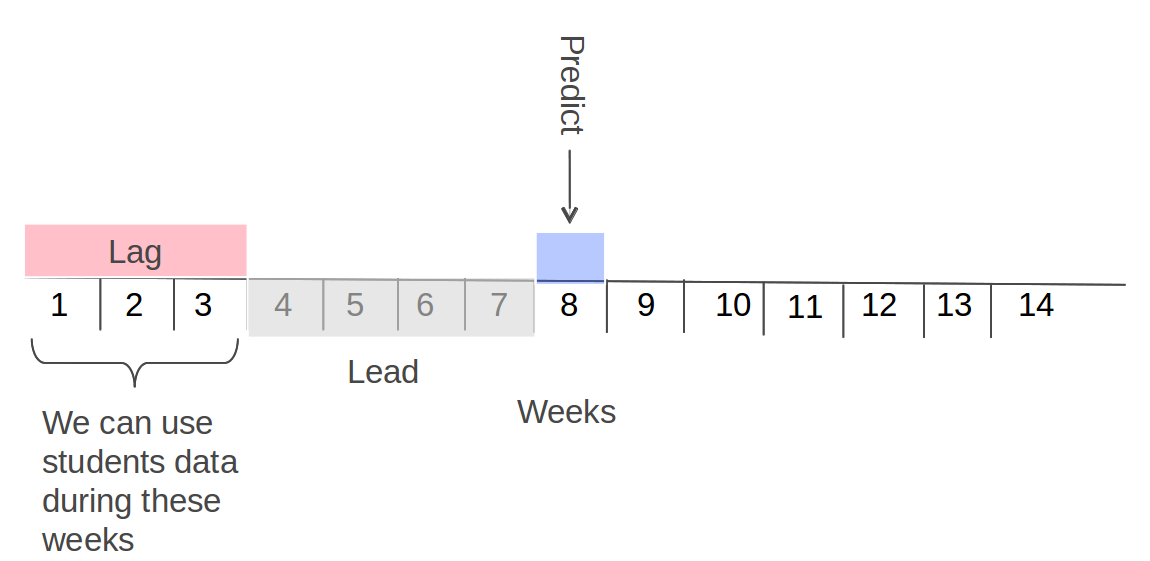
\includegraphics[width=1.0\textwidth]{figures/lead_lag.png}
\end{figure}

We are careful not to use students' stopped out week's features as input to our models. In other words, if a student has stopped out in week 1, 2 or 3, we do not use this student as a data point. Including stopped out student data makes the classification problem too easy as the model will learn that a stopped out student never returns (by our \sti definition).

\section{Dataset partitioning into cohorts}
Rather than treat all students uniformly, we decided to build predictive models for different types of students. With this in mind we divided the students into cohorts as a rough surrogate variable for their commitment to the course. We chose four cohorts based on the student’s collaborative activity throughout the course. More specifically, we divided students based on whether or not they participated in the class forum or helped edit the class Wiki pages. The four types of students are:

\begin{itemize}
\item \neither - these students never actively participated in either the forum or the Wiki. They are named passive because they passively viewed, but did not contribute to, resources.
\item \wiki - these students actively participated in the Wiki by generating Wiki content through their edits, but never actively posted in the forum.
\item \forum - these students actively posted in the forum, but never actively participated in the class Wiki.
\item \both - these students actively participated by generating Wiki content and by posting in the forum
\end{itemize}

From the combined dataset of 52,939 participating students, we assigned each student into one of the four types. The following chart summarizes the sizes of the cohort datasets.

\begin{figure}[!ht]
  \caption{Chart of the relative sizes of our cohorts}\label{fig:cohort_split}
  \centering
    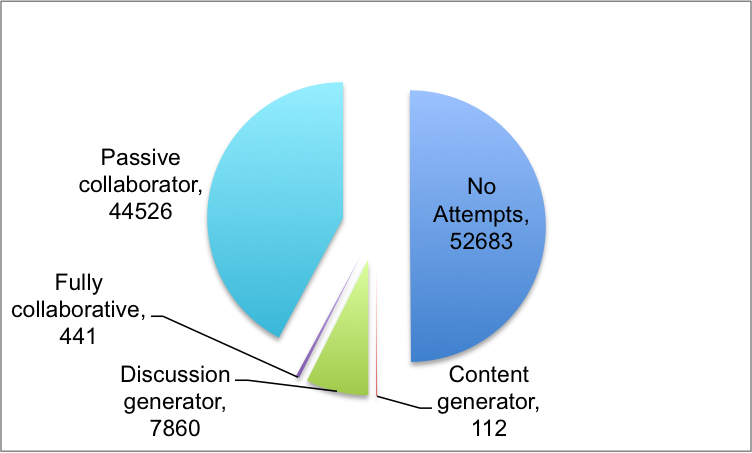
\includegraphics[width=1.0\textwidth]{figures/cohort_split.png}
\end{figure}

For all of the ensuing modelling and analysis, we treated and reported on each of the cohort datasets independently.
